\documentclass[11pt,english,dvipsnames,aspectratio=169,handout]{beamer}\usepackage[]{graphicx}\usepackage[]{xcolor}
% maxwidth is the original width if it is less than linewidth
% otherwise use linewidth (to make sure the graphics do not exceed the margin)
\makeatletter
\def\maxwidth{ %
  \ifdim\Gin@nat@width>\linewidth
    \linewidth
  \else
    \Gin@nat@width
  \fi
}
\makeatother

\definecolor{fgcolor}{rgb}{0.345, 0.345, 0.345}
\newcommand{\hlnum}[1]{\textcolor[rgb]{0.686,0.059,0.569}{#1}}%
\newcommand{\hlstr}[1]{\textcolor[rgb]{0.192,0.494,0.8}{#1}}%
\newcommand{\hlcom}[1]{\textcolor[rgb]{0.678,0.584,0.686}{\textit{#1}}}%
\newcommand{\hlopt}[1]{\textcolor[rgb]{0,0,0}{#1}}%
\newcommand{\hlstd}[1]{\textcolor[rgb]{0.345,0.345,0.345}{#1}}%
\newcommand{\hlkwa}[1]{\textcolor[rgb]{0.161,0.373,0.58}{\textbf{#1}}}%
\newcommand{\hlkwb}[1]{\textcolor[rgb]{0.69,0.353,0.396}{#1}}%
\newcommand{\hlkwc}[1]{\textcolor[rgb]{0.333,0.667,0.333}{#1}}%
\newcommand{\hlkwd}[1]{\textcolor[rgb]{0.737,0.353,0.396}{\textbf{#1}}}%
\let\hlipl\hlkwb

\usepackage{framed}
\makeatletter
\newenvironment{kframe}{%
 \def\at@end@of@kframe{}%
 \ifinner\ifhmode%
  \def\at@end@of@kframe{\end{minipage}}%
  \begin{minipage}{\columnwidth}%
 \fi\fi%
 \def\FrameCommand##1{\hskip\@totalleftmargin \hskip-\fboxsep
 \colorbox{shadecolor}{##1}\hskip-\fboxsep
     % There is no \\@totalrightmargin, so:
     \hskip-\linewidth \hskip-\@totalleftmargin \hskip\columnwidth}%
 \MakeFramed {\advance\hsize-\width
   \@totalleftmargin\z@ \linewidth\hsize
   \@setminipage}}%
 {\par\unskip\endMakeFramed%
 \at@end@of@kframe}
\makeatother

\definecolor{shadecolor}{rgb}{.97, .97, .97}
\definecolor{messagecolor}{rgb}{0, 0, 0}
\definecolor{warningcolor}{rgb}{1, 0, 1}
\definecolor{errorcolor}{rgb}{1, 0, 0}
\newenvironment{knitrout}{}{} % an empty environment to be redefined in TeX

\usepackage{alltt}
\usepackage{fontspec}
\setsansfont[Mapping=tex-text]{Fira Sans}
\setcounter{secnumdepth}{4}
\setcounter{tocdepth}{4}
\usepackage[normalem]{ulem}
\usepackage[T1]{fontenc}
\usepackage{dcolumn}
\usepackage{booktabs}
\usepackage{bm}
\usepackage{setspace}
\makeatletter
\usetheme{metropolis}
\setbeamertemplate{frame footer}{Bosancianu | Schaub | Hertie School}
\setbeamerfont{page number in head/foot}{size=\tiny}
\setbeamercolor{footline}{fg=gray}
\usepackage{xcolor}
\setbeamercovered{dynamic}
\usepackage{tikz}
\usetikzlibrary{arrows, positioning,fit,shapes.misc}
\usepackage[labelformat=empty]{caption}
% For table captions in Beamer
\usepackage[sectionbib]{apacite}
\renewcommand{\bibliographytypesize}{\footnotesize}
\makeatletter
\let\st@rtbibsection\@bibnewpage
\let\st@rtbibchapter\@bibnewpage
\makeatother
\usepackage{amsmath, mathtools}
\usepackage{xunicode}
\usepackage{hyperref}
\usepackage{pgfplots}
\makeatletter
\long\def\ifnodedefined#1#2#3{%
    \@ifundefined{pgf@sh@ns@#1}{#3}{#2}%
}
\pgfplotsset{
    discontinuous/.style={
    scatter,
    scatter/@pre marker code/.code={
        \ifnodedefined{marker}{
            \pgfpointdiff{\pgfpointanchor{marker}{center}}%
             {\pgfpoint{0}{0}}%
             \ifdim\pgf@y>0pt
                \tikzset{options/.style={mark=*}}
                \draw [densely dashed] (marker-|0,0) -- (0,0);
                \draw plot [mark=*,mark options={fill=white}] coordinates {(marker-|0,0)};
             \else
                \ifdim\pgf@y<0pt
                    \tikzset{options/.style={mark=*,fill=white}}
                    \draw [densely dashed] (marker-|0,0) -- (0,0);
                    \draw plot [mark=*] coordinates {(marker-|0,0)};
                \else
                    \tikzset{options/.style={mark=none}}
                \fi
             \fi
        }{
            \tikzset{options/.style={mark=none}}        
        }
        \coordinate (marker) at (0,0);
        \begin{scope}[options]
    },
    scatter/@post marker code/.code={\end{scope}}
    }
}
\makeatother
% Defines a checkmark
\def\checkmark{\tikz\fill[scale=0.4,color=orange](0,.35) -- (.25,0) -- (1,.7) -- (.25,.15) -- cycle;}
\newcommand{\indep}{\perp \!\!\!\! \perp}
\setbeamertemplate{itemize items}{\checkmark}
\usepackage{multirow}
\hypersetup{pdfauthor={Bosancianu and Schaub},
	pdftitle={Statistical Modeling and Causal Inference with R},
	pdfsubject={Week 9: Panel Data},
	pdfkeywords={Berlin, Hertie, 2020, week 9, RDD}}
\title{\textsc{Statistical Modeling and Causal Inference with R}}
\subtitle{Week 9: Panel Data}
\date{November 9, 2020}
\author{Manuel Bosancianu \hfill Max Schaub}
\institute{Hertie School of Governance}
\IfFileExists{upquote.sty}{\usepackage{upquote}}{}
\begin{document}
\maketitle

\begin{frame}
	\frametitle{Recap}
  A powerful way to achieve causal identification: leverage multiple observations over time.\bigskip
  \pause
  
  The DiD estimator manages to do this with 2 observations in time: prior to and after a treatment was applied.\bigskip
  \pause
  
  Excellent at ensuring that unobserved time-invariant confounders don't bias estimates (comparisons happen within-units).\bigskip
  \pause
  
  Assumption: \textcolor{orange}{parallel trends}. Had there been no treatment, temporal dynamics for treatment group would have been the same as for control group.

\end{frame}




\begin{frame}
\frametitle{Parallel trends}

\begin{columns}
	\begin{column}{0.35\textwidth}
	Effect: $Y_{t=2}^{A} - Y_{t=2}^{A^{'}}$\bigskip
	
	Not mandatory to have same units over time---works for pooled cross-sections too.
	\end{column}
	\begin{column}{0.65\textwidth}
		\begin{tikzpicture}[scale = 0.9]

\begin{axis}[
    samples=11,
    jump mark left,
    ymin=0,ymax=1,
    xmin=0, xmax=10,
    every axis plot/.style={very thick},
    discontinuous
]
\node[label=left:{\tiny{$A_{t=1}$}}] at (axis cs:2,0.8) [circle, scale=0.5, draw=black!80] {};
\node[label=left:{\tiny{$B_{t=1}$}}] at (axis cs:2,0.6) [circle, scale=0.5, draw=black!80] {};
\node[label=right:{\tiny{$A_{t=2}$}}] at (axis cs:6,0.7) [circle, scale=0.5, draw=black!80, fill=black!80] {};
\node[label=right:{\tiny{$B_{t=2}$}}] at (axis cs:6,0.3) [circle, scale=0.5, draw=black!80] {};
\draw [thick, -] (axis cs: 2,0.8) -- (axis cs: 6,0.7) node {}; 
\draw [thick, -] (axis cs: 2,0.6) -- (axis cs: 6,0.3) node {}; 
\draw [thick, -, dotted] (axis cs: 2,0.8) -- (axis cs: 6,0.5) node {}; 
\node[label=right:{\tiny{$A_{t=2}^{'}$}}] at (axis cs:6,0.5) [circle, dotted, scale=0.5, draw=black!80, fill=gray!80] {};
\end{axis}
\end{tikzpicture}
	\end{column}
\end{columns}
\pause

\begin{center}
$\beta = (Y_{t=2}^{A} - Y_{t=2}^{B}) - (Y_{t=1}^{A} - Y_{t=1}^{B})$
\end{center}

\end{frame}


\begin{frame}
	\frametitle{Today's plan}
	Extend this design to cases with more than 2 time points:
	
	\begin{itemize}
	\setlength\itemsep{1.5em}
	\item Features of 2 ``pure'' designs: cross-sectional and temporal;
	\item Panel data as a mix of CS and T;
	\item Estimation: \texttt{FE} vs. \texttt{RE}
	\item Assumptions implicit in strategies
	\end{itemize}
	
\end{frame}


\section{Cross-sectional and temporal designs}

\begin{frame}
  \frametitle{Types of data structures}
  \textbf{Cross-section}: sample of countries, firms, regions, schools, employees \dots\ all measured at same time point, \textit{t}.
  
  Measurements on $(Y_i; X_i)$ for $i = 1, 2, \dots, N$ at time \textit{t}.\bigskip
  \pause
  
  \textbf{Time-series}: same unit (country, school, firm, child) measured over multiple time points.
  
  Measurements on $(Y_t; X_t)$ for $t = 1, 2, \dots, T$ for same unit.
  
\end{frame}


\begin{frame}
  \frametitle{Types of data structures}
  \textbf{Panel data}: multiple units measured over multiple time points.
  
  Measurements on $(Y_{it}; X_{it})$ for $i = 1, 2, \dots, N$, and $t = 1, 2, \dots, T$.\bigskip
  \pause
  
  ``Pure'' CS or TS designs have weaknesses in terms of ability to estimate a causal effect.\bigskip
  
  Panel data can (theoretically) overcome these weaknesses.
  
\end{frame}

\begin{frame}
  \frametitle{Short didactic example}
  \citeA{card_minimum_1994} examine whether a minimum price increase influences unemployment.\bigskip
  \pause

  Treatment: increase in minimum wage in NJ (but not in PA) in Apr. 1992.



  Same restaurants over time---Feb. 1992 and Nov.-Dec. 1992.

\end{frame}

\subsection{Cross-sectional}
\begin{frame}
  \frametitle{Static-group comparison}
  
  \begin{align*}
  Y_{i1}^0 &= \theta_{i}^0 + \delta_1 + \upsilon_{i1}^0\\
  Y_{i1}^1 &= \tau + \theta_{i}^1 + \delta_1 + \upsilon_{i1}^1
\end{align*}
  
  $\theta_i$: time-invariant unit-specific effect.
  
  $\delta_t$: time period effect (identical for all units here: $\delta_1$).
  \pause
  
  \begin{equation}
    \centering
    E[Y_{i1}^1 - Y_{i1}^0] = \tau + E[\theta_{i}^1 - \theta_{i}^0] + E[\upsilon_{i1}^1 - \upsilon_{i1}^0]
  \end{equation}
  
  $\delta_1$ disappears---unobserved time-varying factors don't bias the estimate.
  
\end{frame}


\begin{frame}
\frametitle{Assumptions made}
  \textcolor{orange}{Exogeneity}: mean of error is independent of the treatment.
  
  \begin{equation}
    \centering
    E[\upsilon_{i}^1] = E[\upsilon_{i}^0] \Rightarrow E[\upsilon_{i}^1 - \upsilon_{i}^0] = 0
  \end{equation}
  \pause
  
  \textcolor{orange}{Random effects}: unobserved unit heterogeneity is independent of the treatment.

  \begin{equation}
    \centering
    E[\theta_{i}^1] = E[\theta_{i}^0] \Rightarrow E[\theta_{i}^1 - \theta_{i}^0] = 0
  \end{equation}
\end{frame}


\begin{frame}
\frametitle{Effect of wage increase: static comparison}
  If we're willing to make the two assumptions, a static comparison can recover treatment effect.\bigskip
  

\begin{table}
\caption{Model for employment change (Nov. 1992 data)}
\begin{center}
\begin{tiny}
\begin{tabular}{l D{.}{.}{3.5}}
\toprule
 & \multicolumn{1}{c}{DV: No. full-time} \\
\midrule
(Intercept) & 7.56^{***} \\
            & (0.91)     \\
State (NJ)  & 0.88       \\
            & (1.01)     \\
\midrule
R$^2$       & 0.00       \\
Adj. R$^2$  & -0.00      \\
Num. obs.   & 398        \\
\bottomrule
\multicolumn{2}{l}{\tiny{$^{***}p<0.001$; $^{**}p<0.01$; $^{*}p<0.05$}}
\end{tabular}
\end{tiny}
\label{tab:01}
\end{center}
\end{table}

  
  \pause
  
Heroic random effects assumption---even with controls, hard to make it convincing.

\end{frame}




\subsection{Longitudinal}

\begin{frame}
\frametitle{Longitudinal comparison}
 \begin{align*}
  Y_{i0}^0 &= \delta_{0}^0 + \theta_i + \upsilon_{i0}^0\\
  Y_{i1}^1 &= \tau + \delta_{1}^1 + \theta_i + \upsilon_{i1}^1
\end{align*}
  
  $\theta_i$: time-invariant unit-specific effect (identical for all units here).
  
  $\delta_t$: time period effect.
  \pause
  
   \begin{equation}
    \centering
    E[Y_{i1}^1 - Y_{i0}^0] = \tau + E[\delta_{1}^1 - \delta_{0}^0] + E[\upsilon_{i1}^1 - \upsilon_{i1}^0]
  \end{equation}
  
  $\theta_i$ disappears---unobserved time-invariant unit-specific effect don't bias estimate.

\end{frame}


\begin{frame}
\frametitle{Assumptions made}
  \textcolor{orange}{Exogeneity}: $E[\upsilon_{i1}^1] = E[\upsilon_{i0}^0]$.\bigskip
  \pause
  
  \textcolor{orange}{Temporal stability}: no impact of unobserved time-varying factors.

  \begin{equation}
    \centering
    E[\delta_{1}^1] = E[\delta_{0}^0]
  \end{equation}
  \pause
  
  Time-invariant factors ($\theta_i$) don't matter, because the units compared are the same.
\end{frame}


\begin{frame}
\frametitle{Effect of wage increase: temporal comparison}


\begin{table}
\caption{Model for employment change (NJ data)}
\begin{center}
\begin{tiny}
\begin{tabular}{l D{.}{.}{3.5}}
\toprule
 & \multicolumn{1}{c}{DV: No. full-time} \\
\midrule
(Intercept)      & 7.72^{***} \\
                 & (0.44)     \\
Time (Nov. 1992) & 0.72       \\
                 & (0.62)     \\
\midrule
R$^2$            & 0.00       \\
Adj. R$^2$       & 0.00       \\
Num. obs.        & 647        \\
\bottomrule
\multicolumn{2}{l}{\tiny{$^{***}p<0.001$; $^{**}p<0.01$; $^{*}p<0.05$}}
\end{tabular}
\end{tiny}
\label{tab:02}
\end{center}
\end{table}

  
  \pause
  
Heroic temporal stability assumption.

\end{frame}


\section{Panel Data}

\begin{frame}
	\frametitle{Benefits}
	Partly addresses the unit heterogeneity and temporal instability problems.\bigskip
	
	Relies on a weaker exogeneity assumption.\pause
	
	\begin{equation}
	  \footnotesize
	  E[Y_{i1}^1 - Y_{i1}^0] - E[Y_{i0}^1 - Y_{i0}^0] = \tau + E[\epsilon_{i1}^1 - \epsilon_{i1}^0] - E[\epsilon_{i0}^1 - \epsilon_{i0}^0]
	\end{equation}
	
	You saw this in previous class: DiD estimator was applied to a specific type of panel data.\bigskip
	\pause
	
	Extending the lessons of DiD to instances with $t>2$ and where, typically, $N \gg T$.
	
\end{frame}


\begin{frame}
	\frametitle{General structure}
	
	\begin{equation}
	  \centering
	  Y_{it} = \beta_0 + \beta_1D_{it} + \underbrace{\theta_i + \delta_t + \upsilon_{it}}_{\epsilon_{it}}
	\end{equation}\bigskip
	\pause
	
	Error term components:
	
	\begin{itemize}
	\item $\theta_i$: unit fixed effect---captures influence of time-invariant features\pause
	\item $\delta_t$: time fixed effect---captures influence of time-varying features (affect all units)\pause
	\item $\epsilon_{it}$: ``classical'' error term
	\end{itemize}
	
\end{frame}


\begin{frame}
	\frametitle{Benefits of panel data I}
	
	\begin{equation}
	  \centering
	  Y_{it} = \beta_0 + \beta_1D_{it} + \underbrace{\theta_i + \delta_t + \upsilon_{it}}_{\epsilon_{it}}
	\end{equation}
	
	Normally, in this setup, \textcolor{orange}{homogeneity} assumption is violated: $Cov(D_{it}, \theta_i) \neq 0$.\bigskip
	\pause
	
	However, we can partial out $\theta_i$ from $\epsilon_{it}$ (it's constant in longitudinal data) by ``taking out'' unit means in the outcome.

\end{frame}


\begin{frame}
\frametitle{Partialling out $\theta_i$}

\begin{figure}[scale=0.8]
\centering
\begin{tikzpicture}
\begin{axis}[
xlabel=Time (days), % label x axis
ylabel=Y (outcome), % label y axis
axis lines=left, %set the position of the axes
xmin=0, xmax=70, % set the min and max values of the x-axis
ymin=0, ymax=50, % set the min and max values of the y-axis
clip=false
]

\node [circle, fill=orange, scale=0.3, label={$I_{11}$}] (A) at (axis cs: 8, 35) {};
\node [circle, fill=orange, scale=0.3, label={$I_{12}$}] (C) at (axis cs: 35, 15) {};
\node [circle, fill=orange, scale=0.3, label={$I_{13}$}] (E) at (axis cs: 55, 10) {};
\node [circle, fill=black, scale=0.3, label={$I_{21}$}] (B) at (axis cs: 8, 43) {};
\node [circle, fill=black, scale=0.3, label={$I_{22}$}] (F) at (axis cs: 35, 40) {};
\node [circle, fill=black, scale=0.3, label={$I_{23}$}] (D) at (axis cs: 55, 19) {};
\node [circle, scale=0.7] (T1) at (axis cs: 15, 10) {\tiny For $I_{11}$, Y=35};
\node [circle, scale=0.7] (T2) at (axis cs: 15, 8) {\tiny For $I_{12}$, Y=15};
\node [circle, scale=0.7] (T3) at (axis cs: 15, 6) {\tiny For $I_{13}$, Y=10};
\node [circle, scale=0.7] (T4) at (axis cs: 25, 50) {\tiny For $I_{21}$, Y=43};
\node [circle, scale=0.7] (T5) at (axis cs: 25, 48) {\tiny For $I_{22}$, Y=40};
\node [circle, scale=0.7] (T6) at (axis cs: 25, 46) {\tiny For $I_{23}$, Y=19};
%\draw [very thick, red, dashed] (axis cs:5,35)--(axis cs:55,10);
\end{axis}
\end{tikzpicture}
\end{figure}

\end{frame}


\begin{frame}
\frametitle{Partialling out $\theta_i$}
For group 1, $\overline{Y}$=20. For group 2, $\overline{Y}$=35. \bigskip

\begin{table}
\centering
\begin{tabular}{l c c}
\toprule
    & Y raw & $\theta_i$ partialled out \\
\midrule
$I_{11}$ & 35 & 15 \\
$I_{12}$ & 15 & -5 \\
$I_{13}$ & 10 & -10 \\
\midrule
$I_{21}$ & 43 & 8 \\
$I_{22}$ & 40 & 5 \\
$I_{23}$ & 19 & -16 \\
\bottomrule
\end{tabular}
\end{table}
\bigskip
\pause

Remaining variance is the relative position of units within a group, e.g. the distance between $I_{11}$ and $I_{12}$ is still 20.
\end{frame}


\begin{frame}
	\frametitle{Benefits of panel data II}
	
	\begin{equation}
	  \centering
	  Y_{it} = \beta_0 + \beta_1D_{it} + \underbrace{\theta_i + \delta_t + \upsilon_{it}}_{\epsilon_{it}}
	\end{equation}
	
	\textcolor{orange}{Temporal stability} assumption is violated as well: $Cov(D_{it}, \delta_t) \neq 0$.\bigskip
	\pause
	
	We can partial out $\delta_t$ from $\epsilon_{it}$ (it's constant in cross-sectional) by ``taking out'' period means in the outcome.

\end{frame}


\begin{frame}
\frametitle{Same panel setup}

\begin{figure}[scale=0.8]
\centering
\begin{tikzpicture}
\begin{axis}[
xlabel=Time (days), % label x axis
ylabel=Y (outcome), % label y axis
axis lines=left, %set the position of the axes
xmin=0, xmax=70, % set the min and max values of the x-axis
ymin=0, ymax=50, % set the min and max values of the y-axis
clip=false
]

\node [circle, fill=orange, scale=0.3, label={$I_{11}$}] (A) at (axis cs: 8, 35) {};
\node [circle, fill=orange, scale=0.3, label={$I_{12}$}] (C) at (axis cs: 35, 15) {};
\node [circle, fill=orange, scale=0.3, label={$I_{13}$}] (E) at (axis cs: 55, 10) {};
\node [circle, fill=black, scale=0.3, label={$I_{21}$}] (B) at (axis cs: 8, 43) {};
\node [circle, fill=black, scale=0.3, label={$I_{22}$}] (F) at (axis cs: 35, 40) {};
\node [circle, fill=black, scale=0.3, label={$I_{23}$}] (D) at (axis cs: 55, 19) {};
\node [circle, scale=0.7] (T1) at (axis cs: 15, 10) {\tiny For $I_{11}$, Y=35};
\node [circle, scale=0.7] (T2) at (axis cs: 15, 8) {\tiny For $I_{12}$, Y=15};
\node [circle, scale=0.7] (T3) at (axis cs: 15, 6) {\tiny For $I_{13}$, Y=10};
\node [circle, scale=0.7] (T4) at (axis cs: 25, 50) {\tiny For $I_{21}$, Y=43};
\node [circle, scale=0.7] (T5) at (axis cs: 25, 48) {\tiny For $I_{22}$, Y=40};
\node [circle, scale=0.7] (T6) at (axis cs: 25, 46) {\tiny For $I_{23}$, Y=19};
%\draw [very thick, red, dashed] (axis cs:5,35)--(axis cs:55,10);
\end{axis}
\end{tikzpicture}
\end{figure}

\end{frame}


\begin{frame}
\frametitle{Partialling out $\delta_t$}
$\overline{Y}_{period\; 1}=39$ | $\overline{Y}_{period\; 2}=27.5$ | $\overline{Y}_{period\; 3}=14.5$. \bigskip

\begin{table}
\centering
\begin{tabular}{l c c}
\toprule
    & Y raw & $\delta_t$ partialled out \\
\midrule
$I_{11}$ & 35 & -4 \\
$I_{21}$ & 43 & 4 \\
\midrule
$I_{12}$ & 15 & -12.5 \\
$I_{22}$ & 40 &  12.5 \\
\midrule
$I_{13}$ & 10 & -4.5 \\
$I_{23}$ & 19 &  4.5 \\
\bottomrule
\end{tabular}
\end{table}
\bigskip
\pause

Remaining variance is the relative position of units within a time period, e.g. the distance between $I_{11}$ and $I_{21}$ is still 8.
\end{frame}


\begin{frame}
\frametitle{DiD redux I}
We will cover the mechanics of partialling out $\theta_i$ and $\delta_t$ in the next section: \textit{Estimation}.\bigskip

See how similar this is to the \texttt{DiD} framework!\bigskip
\pause

\begin{equation}
  Y_{ct} = \alpha + \beta D_c + \gamma Post_t + \tau (D_c \times Post_t) + \upsilon_{ct}
\end{equation}
\pause

$D_c$: partials out unit heterogeneity.

$Post_t$: partials out temporal instability.


\end{frame}


\begin{frame}
\frametitle{DiD redux II}

\begin{equation}
  Employment_{it} = \alpha + \underbrace{\beta State_i}_{\theta_i} + \underbrace{\gamma Time_t}_{\delta_t} + \tau (State_i \times Time_t) + \upsilon_{it}
\end{equation}
\pause

$State_i \times Time_t$ is an indicator for the treatment:

\begin{equation}
  State_i \times Time_t=\begin{cases}
    1, & \text{if NJ \texttt{AND} Nov. 1992}\\
    0, & \text{if PA \texttt{OR} Feb. 1992}
  \end{cases}
\end{equation}
\pause

\end{frame}


\begin{frame}
\frametitle{Effect of wage increase}


\begin{table}
\caption{Model for employment change}
\begin{center}
\begin{tiny}
\begin{tabular}{l D{.}{.}{3.5}}
\toprule
 & \multicolumn{1}{c}{DV: No. full-time} \\
\midrule
(Intercept)  & 10.21^{***} \\
             & (0.94)      \\
State (NJ)   & -2.48^{*}   \\
             & (1.04)      \\
Time (Nov.)  & -2.64^{*}   \\
             & (1.33)      \\
State x Time & 3.36^{*}    \\
             & (1.48)      \\
\midrule
R$^2$        & 0.01        \\
Adj. R$^2$   & 0.00        \\
Num. obs.    & 802         \\
\bottomrule
\multicolumn{2}{l}{\tiny{$^{***}p<0.001$; $^{**}p<0.01$; $^{*}p<0.05$}}
\end{tabular}
\end{tiny}
\label{tab:03}
\end{center}
\end{table}


Covariates ($X_{it}$) need to be added before jumping to interpretations, but fundamentals are the same.

\end{frame}


\section{Estimation}

\begin{frame}
\frametitle{Simplified set-up}

Let's assume period effects are not a problem (simplifies notation) for now, as it will make the presentation less cumbersome.\bigskip

We're only concerned about unit heterogeneity, $\theta_i$.
\pause

\begin{equation}
  Y_{it} = \beta_0 + \beta_1X_{it} + \theta_i + \upsilon_{it}
\end{equation}\pause

Three strategies to estimate:

\begin{itemize}
  \item first differences (FD)
  \item fixed effects (FE)
  \item random effects (RE)
\end{itemize}

\end{frame}


\begin{frame}
  \frametitle{First differences (FD)}
  
  \begin{align}
  Y_{it} &= \beta_0 + \beta_1X_{it} + \theta_i + \upsilon_{it} \\
  Y_{i(t-1)} &= \beta_0 + \beta_1X_{i(t-1)} + \theta_i + \upsilon_{i(t-1)}
\end{align}\pause

Though $\theta_i$ is a problem, we can eliminate it by differencing.

\begin{align}
  Y_{it} - Y_{i(t-1)} &=  \beta_1X_{it} - \beta_1X_{i(t-1)} + \upsilon_{it} - \upsilon_{i(t-1)} \\
  \Delta Y_{it} &= \beta_1\Delta X_{it} + \Delta\upsilon_{it}
\end{align}
  
\end{frame}


\begin{frame}
  \frametitle{Fixed effects (FE)}
  Alternative is to ``de-mean'' variables, by subtracting their mean across time points.
  
  \begin{align}
  Y_{it} &= \beta_0 + \beta_1X_{it} + \theta_i + \upsilon_{it} \\
  \bar{Y}_{i} &= \beta_0 + \beta_1\bar{X}_i + \bar{\theta_i} + \bar{\upsilon}_i
\end{align}\pause

  Keeping in mind that $\bar{\theta}_i = \frac{\sum_{t=1}^T\theta_i}{T} = \frac{T*\theta_i}{T} = \theta_i$,
  
\begin{equation}
  Y_{it} - \bar{Y}_i = \beta_1(X_{it} - \bar{X}_i) + (\upsilon_{it} - \bar{\upsilon}_i)
\end{equation}

\end{frame}


\begin{frame}
  \frametitle{Dummy variables (LSDV)}
  FE and FD will be mathematically identical \textit{only} in instances with 2 time points.\bigskip
  \pause
  
  Related to FE: Least Squares Dummy Variable (LSDV) regression.\bigskip
  \pause
  
  Logic: use $i-1$ dummy indicators for units, which capture \textit{all} between-unit heterogeneity.

\begin{equation}
  Y_{it} = \beta_0 + \beta_1X_{it} + \underbrace{\beta_2U_1 + \beta_3U_2 + \dots + \beta_iU_{i-1}}_{unit\; dummies} + \upsilon_{it}
\end{equation}\pause

LSDV and FE will be mathematically identical.

\end{frame}


\begin{frame}
  \frametitle{Fixed effects (FE)}
  FE (or LSDV) won't allow the use of time-invariant predictors of $Y_{it}$. They have the same fate as $\theta_i$: de-meaning absorbs them.\bigskip
  \pause
  
  FE can be expanded to also incorporate time-period fixed-effects $\Rightarrow$ \textcolor{orange}{two-way fixed effects}.\bigskip
  \pause
  
  Two-way FE models don't allow for purely time-invariant or purely time-varying predictors; only $X_{it}$ work.

\end{frame}


\begin{frame}
  \frametitle{Random effects (RE)}
  One challenge with LSDV is the large number of parameters estimate (all those unit dummies!).\bigskip
  \pause
  
  Degrees of freedom are: $n*T - n - k$, with $n$ designating units, $T$ time periods, and $k$ covariates; problematic if $T$ is small.\bigskip
  \pause
  
  \begin{equation}
    Y_{it} = \beta_0 + \beta_1X_{it} + \theta_i + \upsilon_{it}
  \end{equation}
  
 \textit{Solution}: avoid estimating $n-1$ coefficients by making a simplifying assumption about distribution of $\theta_i$.
\end{frame}


\begin{frame}
  \frametitle{Random effects (RE)}
  Usually, this assumption is that $\theta_i \sim iid (0, \sigma_{\theta}^2)$.\bigskip
  \pause
  
  In this case, we only estimate a variance (of this distribution).\bigskip
  \pause
  
  Not so much correcting for heterogeneity bias, but \textit{modeling} it.\bigskip
  \pause
  
  However, using the RE estimator requires one strong assumption: $Cov(X_{it}, \theta_i) = 0$, which is encountered rarely in practice.
  
\end{frame}


\section{Assumptions}

\begin{frame}
  \frametitle{Assumptions embedded in FE}
  \citeA{imai_when_2019} refer to the same model, though notation is more complex:
  
  \begin{equation}
    \hat{\beta}_{LIN-FE} = argmin\sum_{i=1}^N\sum_{t=1}^T\{(Y_{it} - \bar{Y}_i) - \beta (X_{it} - \bar{X}_i)\}^2
  \end{equation}\pause
  
  This specification come at the cost of assuming away the possibility of dynamic temporal relationships.
  
\end{frame}



\begin{frame}
  \frametitle{Assumptions of standard FE}
  
  \begin{columns}
  	\begin{column}{0.65\textwidth}
		\begin{figure}
		\centering
		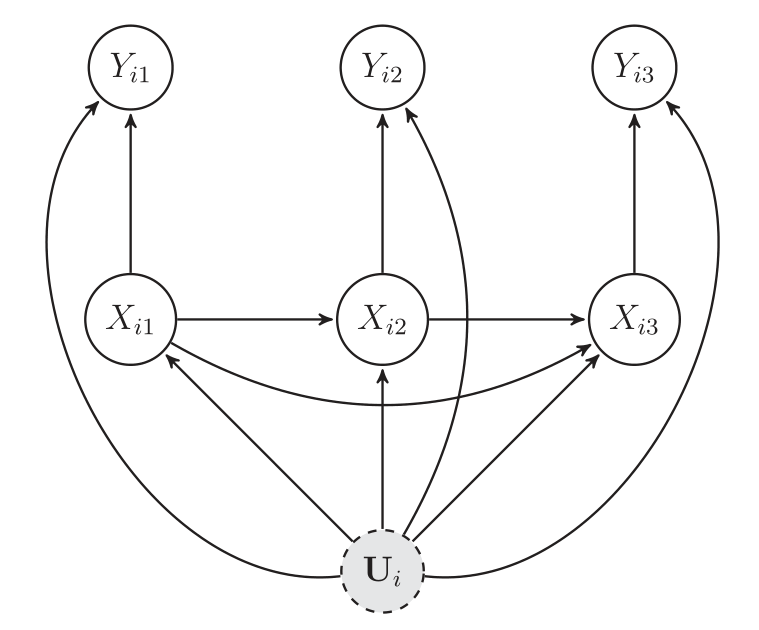
\includegraphics[scale=0.3]{../04-figures/09/01.PNG}
		\end{figure}
	  \end{column}
	\pause
	\begin{column}{0.35\textwidth}
	\footnotesize
	\begin{enumerate}
		\item No unobserved time-varying confounders\pause
		\item Past outcomes don't influence current ones\pause
		\item Past outcomes don't influence current treatment\pause
		\item Past treatment doesn't influence current outcome
	\end{enumerate}
	\end{column}
\end{columns}
  
\end{frame}


\begin{frame}
	\frametitle{Relaxing assumptions I}
	Not much can be done for assumption \#1.\bigskip
	
	\begin{columns}
		\begin{column}{0.65\textwidth}
			\begin{figure}
				\centering
				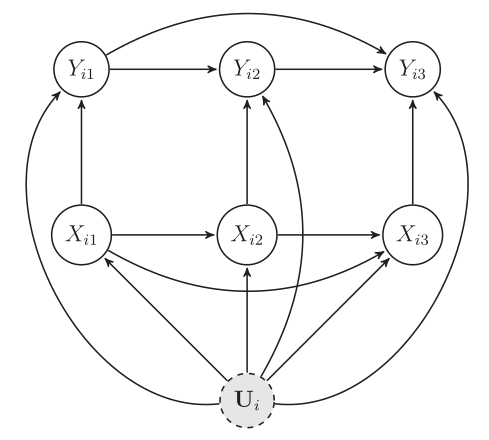
\includegraphics[scale=0.4]{../04-figures/09/02.PNG}
			\end{figure}
		\end{column}
		\begin{column}{0.35\textwidth}
			\footnotesize
				Assumption \#2: $Outcome_{t-1} \nrightarrow Outcome_t$. Can be relaxed without biasing $\tau$.\pause
				
				\begin{equation}
					Y_{it} = \alpha_i + \beta_1X_{it} + \beta_2X_{i(t-1)} + \epsilon_{it}\nonumber
				\end{equation}
		\end{column}
	\end{columns}

\end{frame}


\begin{frame}
	\frametitle{Relaxing assumptions II}
	
	\begin{columns}
		\begin{column}{0.6\textwidth}
			\begin{figure}
				\centering
				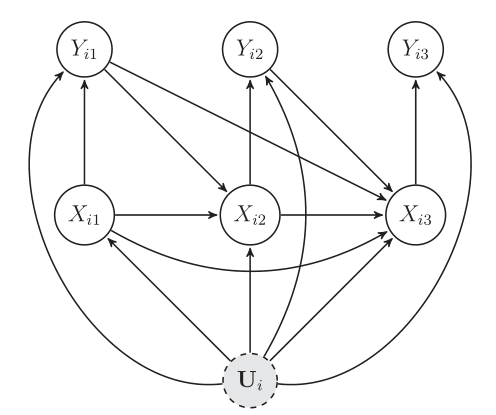
\includegraphics[scale=0.4]{../04-figures/09/03.PNG}
			\end{figure}
		\end{column}
		\begin{column}{0.4\textwidth}
			\footnotesize
			Assumption \#3: $Outcome_{t-1} \nrightarrow Treatment_t$.\pause
			
			\begin{equation}
				Y_{it} = \alpha_i + \beta X_{it} + \rho Y_{i(t-1)} + \epsilon_{it}\nonumber
			\end{equation}\pause
		
		Standard OLS isn't good here (can bias downwards other $\beta$s) \cite{achen_why_2000}.\bigskip\pause
		
		IV-based approach using $X_{i1}$, $X_{i2}$ and $Y_{i1}$ as instruments and controlling for $U_i$ and $Y_{i2}$ \cite{arellano_tests_1991}.
		\end{column}
	\end{columns}
	
\end{frame}

\begin{frame}
	\frametitle{Relaxing assumptions III}
	
	\begin{columns}
		\begin{column}{0.6\textwidth}
			\begin{figure}
				\centering
				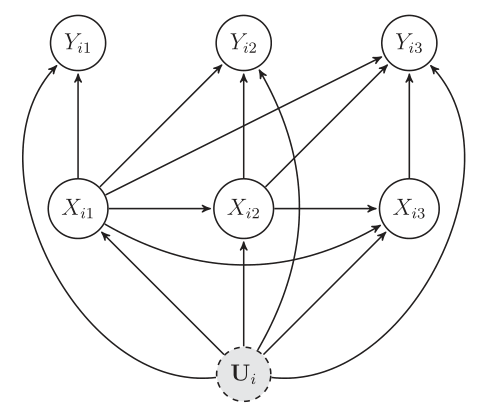
\includegraphics[scale=0.4]{../04-figures/09/04.PNG}
			\end{figure}
		\end{column}
		\begin{column}{0.4\textwidth}
			\footnotesize
			Assumption \#4: $Treatment_{t-1} \nrightarrow Outcome_t$.\pause
			
			\begin{equation}
				Y_{it} = \alpha_i + \beta_1X_{it} + \beta_2X_{i(t-1)} + \epsilon_{it}\nonumber
			\end{equation}\pause
			
			Also dealt with lagged values of predictors (usually 1-period lag).
		\end{column}
	\end{columns}
	
\end{frame}


\section{Summary}

\begin{frame}
  \frametitle{Panel data analysis}
  Very common type of data, allowing researchers to easily control for confounders.\bigskip
  \pause
  
  Offer some leverage over causal inference, given the temporal ordering of observations.\bigskip
  \pause
  
  Gives leverage over both within-unit change, and across-unit differences.

\end{frame}


\begin{frame}
  \frametitle{Panel data analysis}
  However, keeping heterogeneity bias and temporal instability in check comes at the expense of dynamic relationships.\bigskip
  \pause
  
  Solutions have been found for estimating dynamic and long-run effects, but estimation is not straightforward.\bigskip
  \pause
  
  New strategies are still being proposed: \url{https://papers.ssrn.com/sol3/papers.cfm?abstract_id=3555463}.\bigskip
  \pause

	Remaining challenges: (1) settings where $T$ is long; (2) how to handle ``sluggish'' variables (see \url{https://papers.ssrn.com/sol3/papers.cfm?abstract_id=622581}).

\end{frame}


% END
\begin{frame}
\begin{center}
    \Huge Thank \textcolor{orange}{you} for the kind attention!
\end{center}
\end{frame}

% REFERENCES %

\begin{frame}[allowframebreaks, plain]
\bibliographystyle{apacite}
\scriptsize\bibliography{../Bibliography}
\end{frame}

\end{document}
